\documentclass[11pt,oneside,openany]{report}

\usepackage[a4paper,margin=25mm,headheight=22pt,footskip=14mm]{geometry}
\usepackage{fontspec}
\setmainfont{Latin Modern Roman}
\setsansfont{Latin Modern Sans}
\setmonofont{Latin Modern Mono}
\usepackage{microtype}
\usepackage{setspace}
\setstretch{1.08}
\setlength{\emergencystretch}{2em}
\usepackage{xcolor}
\definecolor{VisionNavy}{HTML}{17243D}
\definecolor{VisionTeal}{HTML}{00A6A6}
\definecolor{VisionBlue}{HTML}{5278A2}
\definecolor{VisionPaper}{HTML}{F2F6FA}
\definecolor{VisionAmber}{HTML}{9C6817}
\definecolor{VisionRed}{HTML}{9B4242}
\definecolor{CodeBg}{HTML}{F3F6FA}
\usepackage{graphicx}
\usepackage{booktabs}
\usepackage{tabularx}
\usepackage{longtable}
\usepackage{array}
\usepackage{enumitem}
\setlist{itemsep=2pt,topsep=4pt,leftmargin=1.6em}
\usepackage{amsmath,amssymb}
\usepackage{listings}
\lstdefinestyle{visioncode}{
  basicstyle=\ttfamily\small,
  backgroundcolor=\color{CodeBg},
  frame=single,
  rulecolor=\color{VisionNavy!15},
  keywordstyle=\color{VisionBlue}\bfseries,
  commentstyle=\color{VisionNavy!65}\itshape,
  stringstyle=\color{VisionTeal!70!black},
  breaklines=true,
  columns=fullflexible,
  keepspaces=true,
  showstringspaces=false,
  xleftmargin=5pt,
  xrightmargin=5pt,
  aboveskip=7pt,
  belowskip=7pt
}
\lstset{style=visioncode}
\usepackage{tikz}
\usetikzlibrary{positioning,arrows.meta,shapes.geometric,fit,calc}
\tikzset{
  vbox/.style={draw=VisionNavy!55,fill=VisionPaper,rounded corners=3pt,align=center,inner sep=6pt,font=\small,text width=2.05cm},
  vboxwide/.style={draw=VisionNavy!55,fill=VisionPaper,rounded corners=3pt,align=center,inner sep=8pt,font=\small,text width=3.1cm},
  vteal/.style={draw=VisionTeal!80!black,fill=VisionTeal!9,rounded corners=3pt,align=center,inner sep=7pt,font=\small,text width=2.45cm},
  vmini/.style={draw=VisionNavy!55,fill=VisionPaper,rounded corners=3pt,align=center,inner sep=4pt,font=\scriptsize,text width=1.65cm},
  vamber/.style={draw=VisionAmber,fill=VisionAmber!9,rounded corners=3pt,align=center,inner sep=7pt,font=\small,text width=2.45cm},
  vflow/.style={-{Stealth[length=2.1mm]},draw=VisionTeal!85!black,thick},
  vsoftflow/.style={-{Stealth[length=2mm]},draw=VisionBlue,thick,dashed}
}
\usepackage{caption}
\captionsetup{font=small,labelfont={bf,color=VisionNavy},skip=7pt}
\usepackage{titlesec}
\titleformat{\chapter}[display]
  {\normalfont\sffamily\bfseries\color{VisionNavy}}
  {\filleft\Large\chaptertitlename\ \thechapter}
  {0.5ex}
  {\titlerule\vspace{1.2ex}\Huge}
  [\vspace{0.8ex}\titlerule]
\titlespacing*{\chapter}{0pt}{-5pt}{22pt}
\titleformat{\section}{\large\sffamily\bfseries\color{VisionNavy}}{\thesection}{0.75em}{}
\titleformat{\subsection}{\normalsize\sffamily\bfseries\color{VisionBlue}}{\thesubsection}{0.75em}{}
\usepackage[most]{tcolorbox}
\newtcolorbox{principlebox}{colback=VisionTeal!5,colframe=VisionTeal!65!black,boxrule=0.6pt,arc=2mm,left=2mm,right=2mm,top=1mm,bottom=1mm}
\newtcolorbox{cautionbox}{colback=VisionAmber!7,colframe=VisionAmber!75!black,boxrule=0.6pt,arc=2mm,left=2mm,right=2mm,top=1mm,bottom=1mm}
\usepackage{fancyhdr}
\pagestyle{fancy}
\fancyhf{}
\fancyhead[L]{\small\sffamily\color{VisionNavy}VisionID AI}
\fancyhead[R]{\small\sffamily\color{VisionNavy}Technical Report}
\fancyfoot[L]{\footnotesize\color{VisionNavy!70}Local-first browser demonstration}
\fancyfoot[R]{\footnotesize\color{VisionNavy!70}Page \thepage}
\renewcommand{\headrulewidth}{0.4pt}
\renewcommand{\headrule}{\hbox to\headwidth{\color{VisionTeal}\leaders\hrule height \headrulewidth\hfill}}
\renewcommand{\footrulewidth}{0pt}
\usepackage[backend=biber,style=numeric,sorting=nyt,maxbibnames=4]{biblatex}
\addbibresource{docs/report/references.bib}
\usepackage[hidelinks]{hyperref}
\hypersetup{
  pdftitle={VisionID AI: Intelligent Person Recognition and Real-Time Object Detection Web Platform},
  pdfauthor={VisionID AI Project},
  pdfsubject={Browser-side computer vision architecture, implementation, privacy, and deployment},
  pdfkeywords={computer vision, face recognition, object detection, React, Vercel, privacy}
}
\usepackage[nameinlink,noabbrev]{cleveref}
\setcounter{secnumdepth}{2}
\setcounter{tocdepth}{2}
\renewcommand{\arraystretch}{1.2}
\newcommand{\product}{\textsf{VisionID AI}}
\newcommand{\score}{\texttt{detectorConfidence}}
\newcommand{\similarity}{\texttt{recognitionSimilarity}}
\newcommand{\code}[1]{\texttt{#1}}

\begin{document}
\begin{titlepage}
  \pagecolor{VisionNavy}\color{white}
  \vspace*{18mm}
  {\sffamily\small\color{VisionTeal}\bfseries COMPUTER VISION SYSTEMS \hfill TECHNICAL DOCUMENTATION\par}
  \vspace{25mm}
  {\sffamily\bfseries\fontsize{34}{40}\selectfont VisionID AI\par}
  \vspace{5mm}
  {\sffamily\Large Intelligent Person Recognition and\par Real-Time Object Detection Web Platform\par}
  \vspace{8mm}
  {\color{VisionTeal}\rule{0.28\textwidth}{2pt}\par}
  \vspace{8mm}
  {\large Architecture, browser inference, QR registration,\par local data design, privacy, testing, and deployment\par}
  \vfill
  
\begin{tikzpicture}[node distance=9mm]
    \node[draw=VisionTeal!70,fill=white!5,rounded corners=4pt,text=white,minimum width=36mm,minimum height=13mm] (cam) {CAMERA FRAME};
    \node[draw=VisionTeal!70,fill=white!5,rounded corners=4pt,text=white,minimum width=36mm,minimum height=13mm,right=of cam] (ai) {LOCAL AI};
    \node[draw=VisionTeal!70,fill=white!5,rounded corners=4pt,text=white,minimum width=36mm,minimum height=13mm,right=of ai] (db) {LOCAL RECORDS};
    \draw[-{Stealth[length=2mm]},thick,VisionTeal] (cam) -- (ai);
    \draw[-{Stealth[length=2mm]},thick,VisionTeal] (ai) -- (db);
  \end{tikzpicture}
  \vspace{8mm}
  {\small Local-first single-device demonstration \hfill Version 1.0 \quad 3 October 2026\par}
\end{titlepage}
\nopagecolor
\color{black}
\pagenumbering{roman}

\chapter*{Executive Summary}
\addcontentsline{toc}{chapter}{Executive Summary}
\product{} is a browser-based computer-vision application for two related but distinct tasks: detecting objects in a camera frame and matching a detected face against identities that were explicitly enrolled by a user on that device. The camera stream, face descriptor records, profiles, settings, and detection history remain within one browser profile. The static website and model assets can be hosted on Vercel; there is no runtime API server or cloud person directory.

The application uses React and TypeScript for its interface, Vite for packaging, Dexie over IndexedDB for local persistence, ZXing Browser for QR scanning, Human for face detection/landmarks/face descriptors, and TensorFlow.js COCO-SSD Lite for object detection. A worker-oriented adapter separates model-specific outputs from the interface. A serial inference loop reports measured latency and frames per second, tracks boxes with temporary IDs, and records deduplicated events. Matching uses an enrolled descriptor set and conservative configurable threshold and ambiguity margin. Low or ambiguous scores remain Unknown.

The design deliberately limits its claims. It is a local demonstration, not authentication, a liveness detector, or an access-control decision system. Lighting, pose, camera, model provenance, and hardware affect results. The bundled HSE FaceRes weights have VGGFace2 training provenance; the upstream dataset terms restrict use to non-commercial research. The repository includes this notice because an open-source code license alone does not remove training-data obligations \cite{vggTerms}. No recognition accuracy or minimum frame rate is claimed.

\begin{principlebox}
\textbf{Operational boundary.} A user must start the camera deliberately. Frames are processed in browser memory and discarded. A face becomes an identity only after separate profile creation, consent, and successful live enrollment. Detector confidence and recognition similarity are different quantities throughout the UI, history, exports, and this report.
\end{principlebox}

\tableofcontents
\listoffigures
\listoftables
\clearpage
\pagenumbering{arabic}

\chapter{Introduction}
Computer vision converts image data into structured descriptions that a program can act on. A frame can be searched for object categories, for a face region, or for visual features that distinguish one enrolled face from another. Those operations are not synonyms. Person detection locates a body-shaped category. Face detection locates a face. Face recognition compares a face representation with a set of reference representations. Object detection locates and classifies items from a model's supported vocabulary.

\product{} combines these capabilities in a single responsive browser console. Its Fusion mode can report an object such as a bottle and a face result in the same inference cycle. The app keeps these result types independent: seeing a person-shaped object does not establish a face identity, and recognizing a face does not imply that an adjacent item belongs to that person. The interface shows boxes, class names, temporary tracks, typed scores, system state, and local history.

The product emphasizes visible user control. It begins with the camera off. A user can explore explicitly labeled fictional demo records before granting a camera permission. To use identity matching, the person must be added and face samples captured through the enrollment flow. This creates a transparent path from model output to interface result, rather than treating an opaque score as proof of identity.

Real-time processing makes resource cost visible. Model initialization, inference cadence, frame dimensions, measured FPS, and latency all affect responsiveness. The application reports measurements from the current browser session; it does not promise a fixed rate. Browser hosting is useful for a low-infrastructure demonstration, but it also makes local hardware, browser capabilities, and model rights part of the operating conditions.

\chapter{Problem Statement}
A camera-based application must turn unstructured frames into useful, reviewable information without silently converting uncertainty into a confident label. A minimal object detector does not solve the additional problems of QR registration, voluntary face enrollment, conservative identity matching, local data management, camera lifecycle, model distribution, privacy notices, and recoverable errors.

The project addresses the following problem: how can a single-device web application support live detection and opt-in identity matching while remaining deployable as a static Vercel site, keeping frames local, separating incompatible score meanings, and giving a non-specialist user control over the data that the browser stores?

Several constraints shape the solution:
\begin{itemize}
  \item \textbf{No always-on server.} A static Vercel deployment should serve the application and public model assets without requiring a persistent Python process.
  \item \textbf{No invented result.} Missing inference, model failure, and below-threshold identity scores must not produce a fabricated box, confidence, or name.
  \item \textbf{Consent before enrollment.} A QR payload can describe a profile but cannot enroll a face or grant recognition permission.
  \item \textbf{Local data lifecycle.} Profiles, templates, events, settings, cache, and deletion actions have different purposes and must be managed distinctly.
  \item \textbf{Calibrated claims.} Scores are model outputs or matcher similarities, not universal probabilities of correctness.
\end{itemize}

\chapter{Objectives and Success Criteria}
The product objective is a polished, technically maintainable browser system in which the user can start a camera session, observe real object and face results, optionally enroll their own face, inspect events, and delete local records. Its technical objective is to keep replaceable boundaries around the AI engine and repositories so that browser models can be changed without rewriting the interface.

\begin{table}[htbp]
\centering
\caption{Product objectives and observable completion evidence.}
\begin{tabularx}{\textwidth}{>{\raggedright\arraybackslash}p{0.24\textwidth}X}
\toprule
\textbf{Objective} & \textbf{Evidence in the implementation} \\
\midrule
Show real-time vision & Camera console draws returned boxes and lists actual model classes and scores. \\
Restrict identification & Only explicitly stored non-demo descriptors are candidates; unknown and ambiguous results remain distinct. \\
Register people safely & QR/manual input is validated and previewed; identity capture requires a separate consent action. \\
Keep data local & Dexie repositories use IndexedDB; frames are not persisted or uploaded. \\
Support product operations & History, filters, export redaction, model-cache control, demo reset, and clear-all are available. \\
Deploy simply & Vite emits static files with a route rewrite and no application secrets or API service. \\
Make errors recoverable & Camera/model failures provide messages and retry actions rather than a blank page. \\
\bottomrule
\end{tabularx}
\end{table}

The implementation's automated gates include a strict TypeScript build, ESLint, unit tests, integration tests, UI tests, Playwright flows with explicitly labeled deterministic adapters, and a production Vite build. Real-device model behavior remains a separate hardware smoke check; a test fixture is not evidence of detector accuracy.

\chapter{System Overview}
The browser is the execution environment and the privacy boundary. React routes coordinate input and display. The camera service owns permission and track cleanup. The inference adapter translates model outputs into typed face and object results. Matching and tracking are deterministic application logic. Dexie repositories isolate IndexedDB operations. Vercel serves the static application and versioned assets but does not receive session frames or profiles.

\begin{figure}[htbp]
\centering
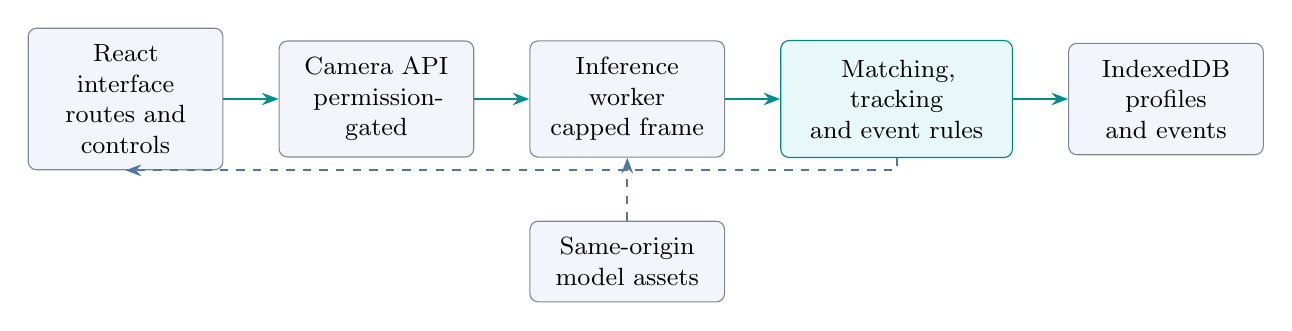
\begin{tikzpicture}[node distance=8mm and 7mm]
  \node[vbox] (ui) {React interface\\routes and controls};
  \node[vbox,right=of ui] (cam) {Camera API\\permission-gated};
  \node[vbox,right=of cam] (worker) {Inference worker\\capped frame};
  \node[vteal,right=of worker] (fusion) {Matching, tracking\\and event rules};
  \node[vbox,right=of fusion] (db) {IndexedDB\\profiles and events};
  \node[vbox,below=of worker] (models) {Same-origin\\model assets};
  \draw[vflow] (ui) -- (cam);
  \draw[vflow] (cam) -- (worker);
  \draw[vflow] (worker) -- (fusion);
  \draw[vflow] (fusion) -- (db);
  \draw[vsoftflow] (models) -- (worker);
  \draw[vsoftflow] (fusion.south) |- (ui.south);
\end{tikzpicture}
\caption{Browser architecture and local processing path. Only public model files are downloaded from the static origin.}
\label{fig:architecture}
\end{figure}

The route set includes an overview, Vision Fusion console, object-only console, enrollment, directory, person profile, history, and settings. Direct route refresh is handled through the static host rewrite. Feature pages are loaded as route chunks, while the model runtime is initialized only when a user starts a vision flow.

\chapter{Technologies Used}
The app uses React 19 for component state and composition, TypeScript 6 for domain contracts, Vite 8 for development and static builds, React Router 7 for route handling, and Tailwind CSS 4 as part of the visual foundation. The exact versions are pinned in the npm lockfile so that a clean install resolves the same dependency graph. React documentation describes the component model used to compose screens and reusable controls \cite{react}; TypeScript adds static checks to those interfaces \cite{typescript}; Vite provides the development server and optimized static output \cite{vite}.

\begin{table}[htbp]
\centering
\caption{Runtime components and selected responsibility.}
\begin{tabularx}{\textwidth}{>{\raggedright\arraybackslash}p{0.31\textwidth}X}
\toprule
\textbf{Component} & \textbf{Role in VisionID AI} \\
\midrule
Human 3.3.6 & Face boxes, landmarks, and 1024-value face descriptors; unrelated attribute modules remain disabled \cite{humanRepo,humanModels}. \\
COCO-SSD 2.2.3 & Lite MobileNet v2 model for the 80 COCO object categories \cite{cocoSsd}. \\
TensorFlow.js 4.22 & Browser model runtime with WebGL, WASM, and CPU fallback paths \cite{tfjs}. \\
Dexie 4.4 & Typed repositories and schema-versioned IndexedDB access \cite{dexie,indexedDb}. \\
ZXing Browser 0.2 & QR camera reading; QR payload text is validated before preview \cite{zxing}. \\
Vitest and Playwright & Fast logic/React checks and isolated browser flow tests. \\
Vercel & Static hosting for built files, model assets, and client-route rewrite \cite{vercelVite}. \\
\bottomrule
\end{tabularx}
\end{table}

Python is intentionally not on the runtime path. The selected inference libraries execute in the browser and allow the application to deploy as static content. A Python toolchain could later support offline evaluation or model conversion, but it would not improve the current single-device deployment boundary enough to justify another service.

\chapter{Computer Vision Fundamentals}
\section{Images, frames, and pixels}
An image is a two-dimensional grid of samples. A video stream is a time-ordered sequence of such images called frames. In an RGB image, each pixel has red, green, and blue channel values. The camera exposes decoded frames through a browser video element; model preprocessing may resize or normalize these channel values before tensor operations. The frame is transient input: the application passes it to the local engine and does not save a snapshot.

\section{Detection, classification, and boxes}
Classification assigns a label to an input. Detection predicts one or more localized instances: a class label and a rectangle around the instance. VisionID represents a box as normalized or pixel-based coordinates depending on the adapter stage. A box is commonly written as \((x,y,w,h)\), where \((x,y)\) marks its top-left corner and \(w,h\) its dimensions. Scaling and aspect ratio matter when the camera frame is resized; overlay drawing maps model coordinates back onto the displayed video.

\section{Confidence, landmarks, and tracking}
A detector score expresses how strongly the model's output favors a class for one box. It is not necessarily a calibrated probability. A face landmark is a predicted keypoint, such as an eye or mouth location, that describes geometry within a detected face. Tracking links boxes between nearby frames and assigns a temporary identifier. In Vision Fusion, a face box can link to a uniquely containing COCO \texttt{person} track; this geometric association is displayed separately and never supplies a face identity. A track ID helps the interface refer to an object for a short time; it is neither a permanent object identity nor a person's identity.

\section{Embeddings}
An embedding or descriptor is a numeric vector produced from a face crop by an embedding model. It represents selected visual features in a model-specific coordinate space. A matcher can compare two vectors using the metric that belongs to that model. VisionID stores descriptors only after explicit enrollment. It does not compare raw image pixels, and it discards the source camera frame after the descriptor is computed.

\begin{principlebox}
Object detector confidence, face detector confidence, and descriptor similarity answer different questions. A large value in one field must not be relabeled as another measure.
\end{principlebox}

\chapter{Face Recognition Pipeline}
The face pipeline starts with a current video frame and returns zero or more face objects. BlazeFace locates face regions. Human's configured face module supplies landmarks and a 1024-value descriptor. The application applies transparent quality checks during enrollment, not as a claim that an image is genuine or live. A passing descriptor is compared with the templates stored for local, consented profiles.

\begin{figure}[htbp]
\centering
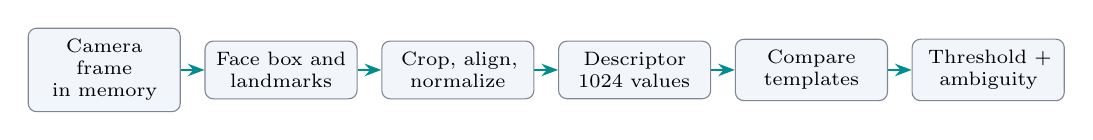
\begin{tikzpicture}[node distance=3mm]
  \node[vmini] (frame) {Camera frame\\in memory};
  \node[vmini,right=of frame] (detect) {Face box and\\landmarks};
  \node[vmini,right=of detect] (prep) {Crop, align,\\normalize};
  \node[vmini,right=of prep] (embed) {Descriptor\\1024 values};
  \node[vmini,right=of embed] (compare) {Compare\\templates};
  \node[vmini,right=of compare] (decision) {Threshold +\\ambiguity};
  \draw[vflow] (frame) -- (detect);
  \draw[vflow] (detect) -- (prep);
  \draw[vflow] (prep) -- (embed);
  \draw[vflow] (embed) -- (compare);
  \draw[vflow] (compare) -- (decision);
\end{tikzpicture}
\caption{Face descriptor extraction and identity decision. A result can remain Unknown.}
\label{fig:face-pipeline}
\end{figure}

Alignment and normalization make the embedding input more consistent with the model's training and expected input geometry. The implementation delegates model-specific preprocessing to Human rather than reimplementing it in a page component. Each frame's detected face is processed independently, so one visible identity cannot be copied to another face in the same frame. Non-enrolled/demo profiles are excluded from candidate lists.

During enrollment the user captures multiple samples at guided front, left, and right prompts. Face count, face size, brightness, sharpness, and pose are checked. These measurements detect obviously poor samples but are not liveness tests. A successfully stored template includes descriptor, model ID, quality score, pose label, and timestamp. Source frame pixels are cleared/discarded.

\chapter{Object Detection Pipeline}
VisionID uses the TensorFlow.js COCO-SSD model with the Lite MobileNet v2 variant. The detector is trained for the COCO category vocabulary, including examples such as person, bottle, chair, cup, laptop, bicycle, and dog. An unsupported item may be missed or assigned a misleading nearby class; the application does not add arbitrary labels through metadata.

\begin{figure}[htbp]
\centering
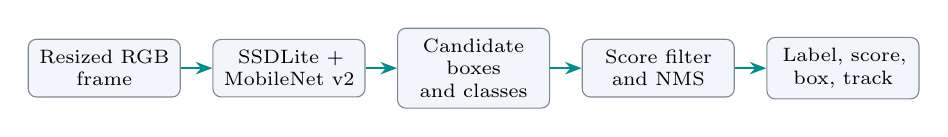
\begin{tikzpicture}[node distance=4mm]
  \node[vmini] (frame) {Resized RGB\\frame};
  \node[vmini,right=of frame] (net) {SSDLite +\\MobileNet v2};
  \node[vmini,right=of net] (candidates) {Candidate boxes\\and classes};
  \node[vmini,right=of candidates] (filter) {Score filter\\and NMS};
  \node[vmini,right=of filter] (view) {Label, score,\\box, track};
  \draw[vflow] (frame) -- (net);
  \draw[vflow] (net) -- (candidates);
  \draw[vflow] (candidates) -- (filter);
  \draw[vflow] (filter) -- (view);
\end{tikzpicture}
\caption{Object output path. COCO-SSD library post-processing supplies candidate detections and non-maximum suppression.}
\label{fig:object-pipeline}
\end{figure}

The runtime resizes frames to configured maximum input dimensions and asks the model for predictions. The COCO-SSD library decodes model outputs and applies its detection post-processing, including suppression of heavily overlapping candidates. The application filters by its configurable object detector threshold, scales returned boxes for presentation, assigns temporary tracks across cycles, and aggregates repeat events. The report does not claim that VisionID itself trains the network or implements the model's internal suppression algorithm.

An object result includes the class label, model class ID, score{}, and bounding box. The details panel adds a temporary track ID and first/last-seen times. The score is a model output. It should be used as an adjustable filtering signal, not as an objective probability of the object being present.

\chapter{QR Architecture}
A QR symbol carries text. For this app, QR text uses versioned JSON so that a human-readable profile can be reviewed before save. The schema requires version 1, a person ID, and a name. It accepts selected bounded text fields and plain metadata. It rejects unsupported root fields, photographs, biometric vectors, malformed data, invalid versions, duplicate IDs (case-insensitive after NFKC normalization), and payloads above 8 KiB UTF-8. The same canonical duplicate rule is checked transactionally when profiles are saved, so stale previews from another tab cannot create conflicting visible IDs.

\begin{figure}[htbp]
\centering
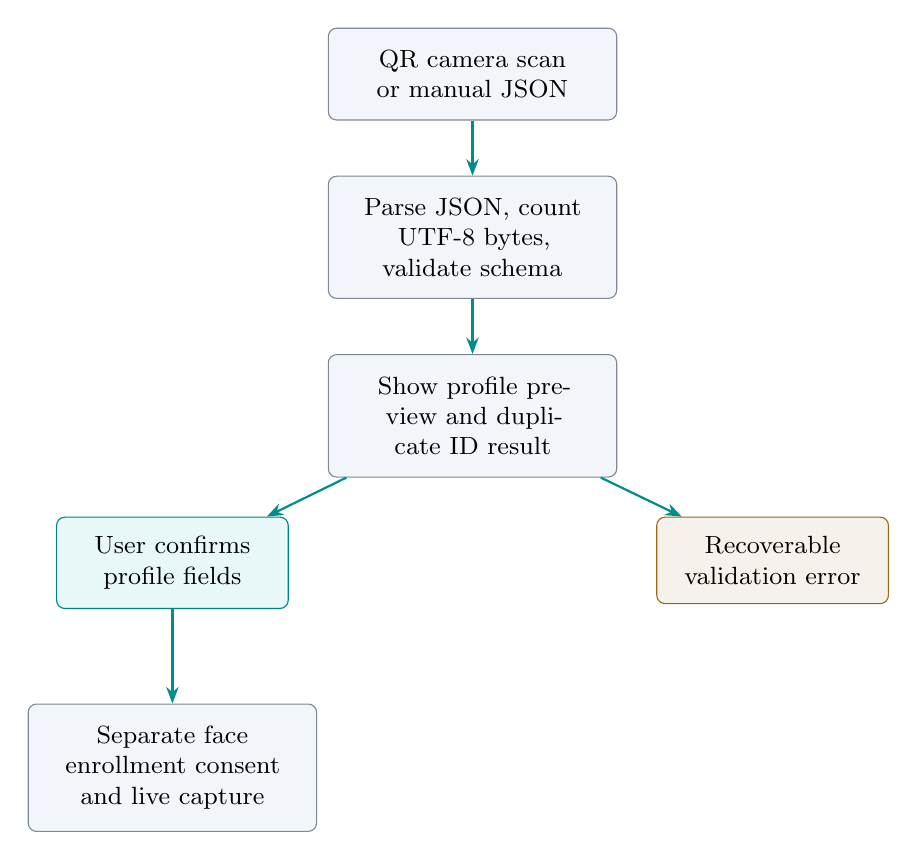
\begin{tikzpicture}[node distance=7mm]
  \node[vboxwide] (input) {QR camera scan or manual JSON};
  \node[vboxwide,below=of input] (parse) {Parse JSON, count UTF-8 bytes, validate schema};
  \node[vboxwide,below=of parse] (review) {Show profile preview and duplicate ID result};
  \node[vteal,below left=of review] (save) {User confirms profile fields};
  \node[vamber,below right=of review] (reject) {Recoverable validation error};
  \node[vboxwide,below=12mm of save] (consent) {Separate face enrollment consent and live capture};
  \draw[vflow] (input) -- (parse);
  \draw[vflow] (parse) -- (review);
  \draw[vflow] (review) -- (save);
  \draw[vflow] (review) -- (reject);
  \draw[vflow] (save) -- (consent);
\end{tikzpicture}
\caption{QR is profile input; it does not skip review or enrollment consent.}
\label{fig:qr-flow}
\end{figure}

The ZXing Browser reader owns camera scan lifecycle and is stopped when the scanner is toggled off or unmounted. The manual paste form uses the same parser and reports the same error types. QR generation serializes only supported profile fields. Camera scanning does not automatically save the payload: the user reviews normalized values in a preview, may cancel, and must separately consent before any face descriptors can be captured.

\begin{lstlisting}[caption={Illustrative v1 payload. This payload describes a profile only.}]
{
  "version": 1,
  "person_id": "P001",
  "name": "Example Person",
  "role": "Student",
  "department": "Computer Science",
  "organization": "Example University",
  "metadata": { "batch": "2026", "section": "A" }
}
\end{lstlisting}

\chapter{Database Design}
Dexie provides a typed interface over the browser's IndexedDB storage. IndexedDB supports structured records and binary blobs without placing large data in localStorage \cite{dexie,indexedDb}. Data is scoped to the browser profile and origin. The application does not replicate records to a remote store.

\begin{figure}[htbp]
\centering
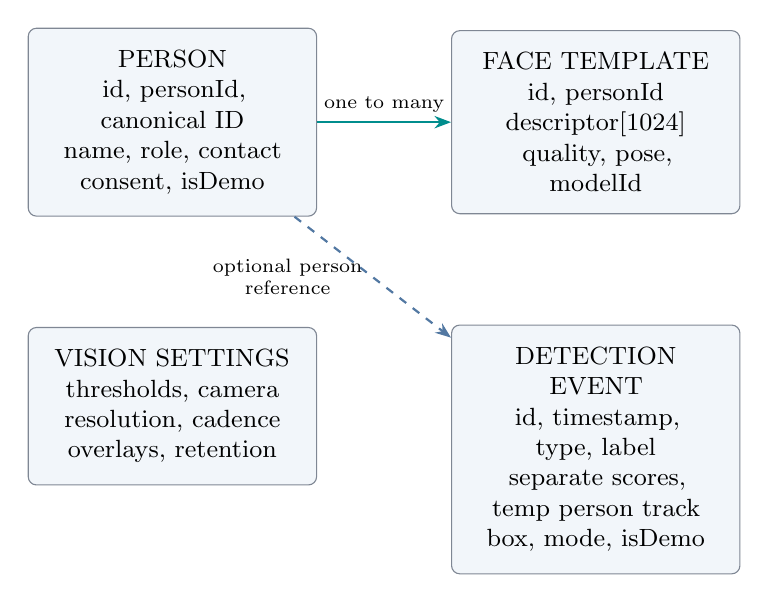
\begin{tikzpicture}[node distance=14mm and 17mm]
  \node[vboxwide] (person) {PERSON\\id, personId, canonical ID\\name, role, contact\\consent, isDemo};
  \node[vboxwide,right=of person] (template) {FACE TEMPLATE\\id, personId\\descriptor[1024]\\quality, pose, modelId};
  \node[vboxwide,below=of template] (event) {DETECTION EVENT\\id, timestamp, type, label\\separate scores, temp person track\\box, mode, isDemo};
  \node[vboxwide,below=of person] (settings) {VISION SETTINGS\\thresholds, camera\\resolution, cadence\\overlays, retention};
  \draw[vflow] (person) -- node[above,font=\scriptsize]{one to many} (template);
  \draw[vsoftflow] (person) -- node[left,font=\scriptsize,align=center]{optional person\\reference} (event);
\end{tikzpicture}
\caption{Core local records. Demo profiles have no face-template rows.}
\label{fig:database}
\end{figure}

\begin{table}[htbp]
\centering
\caption{Stored data and deletion/export policy.}
\begin{tabularx}{\textwidth}{>{\raggedright\arraybackslash}p{0.22\textwidth}XX}
\toprule
\textbf{Store} & \textbf{Purpose} & \textbf{Data boundary} \\
\midrule
Person profile & User-entered identity and contact fields & Local IndexedDB; profile JSON export omits portraits and descriptors. \\
Face template & Enrolled descriptor and sample metadata & Local IndexedDB only; excluded from normal exports; removed with its profile. \\
Detection event & Timestamped local result and typed scores & No frame, face crop, descriptor, or raw QR payload. \\
Settings & Current validated thresholds and preferences & Local IndexedDB; clear-all resets the record. \\
Model cache & Versioned public model and WASM responses & CacheStorage only; separately clearable without personal data loss. \\
\bottomrule
\end{tabularx}
\end{table}

Repositories validate writes and atomically remove linked records when a profile is deleted. Face-template writes check the profile in the same transaction as the template insert. Recognized-event writes also verify linked profiles transactionally and omit events whose profile was deleted; the inference view clears a cached identity if deletion wins before its last-seen update. These checks prevent a late camera result from restoring biometric templates or recognition history after deletion.

\chapter{Frontend Architecture}
The React application is divided by product responsibility rather than screen-shaped monoliths. The app shell owns navigation, skip link, current session status, and the main landmark. Pages and features own their own workflow state. Shared dialogs manage focus, escape, cancellation, and focus return; loading, empty, error, badge, and toast components standardize status without owning persistence.

\begin{table}[htbp]
\centering
\caption{Main frontend responsibilities.}
\begin{tabularx}{\textwidth}{>{\raggedright\arraybackslash}p{0.29\textwidth}X}
\toprule
\textbf{Feature boundary} & \textbf{Responsibilities} \\
\midrule
Landing & Explain the product and camera boundary, link to primary flows, optionally seed fictional demo records. \\
Vision console & Camera stage, overlay, mode controls, model/camera state, current results, latency and FPS. \\
Enrollment & QR/manual entry, review, consent, sample prompts, face-quality report and save. \\
People directory/profile & Search, filters, contact details, recognition history, edit/delete/re-enroll actions. \\
History/dashboard & Event filters, typed score presentation, demo labels, aggregate graphs and redacted downloads. \\
Settings & Bounded config, actual input/cadence presets, retention, model cache and local-data operations. \\
\bottomrule
\end{tabularx}
\end{table}

The major routes are the overview, Fusion console, object console, enrollment, directory, profile detail, history, and settings. They resolve to `/`, `/console`, `/objects`, `/enroll`, `/people`, `/people/:personId`, `/history`, and `/settings`. Route components load lazily to keep the initial JavaScript smaller. The route error boundary provides a recovery link when a page fails. Form fields use native labels, focus is visible, dialogs are keyboard-operable, mobile navigation has a named toggle, and decorative motion follows the reduced-motion preference \cite{wcag}.

\chapter{AI Architecture}
An engine interface describes model initialization, detection, status, configuration, cleanup, and descriptor similarity. The interface returns a `FrameResult` with independent `faces` and `objects` arrays, model ID, inference timing, and warnings. Model-specific fields are normalized once by the adapter. UI components consume application types rather than Human or TensorFlow-specific object shapes.

The worker adapter transfers a downscaled `ImageBitmap` where the browser supports worker inference, then closes it after response. The engine serializes requests to avoid concurrent memory-heavy frames. If worker construction or transfer is unavailable, a main-thread engine uses the same contract. Model file URLs are same-origin and explicitly listed in a versioned manifest with size and SHA-256. Cache writes validate bytes; only allowlisted model/WASM files are cached.

The active Human modules are face detection, landmarks, and face description. Sensitive or unrelated outputs such as age, gender, emotion, race, personality, or health are not enabled. COCO-SSD provides a separate object path with its own label list. Human documents the face embedding and matching interface; the app keeps the final threshold/ambiguity decision in its own matcher \cite{humanEmbedding,humanModels}.

\begin{table}[htbp]
\centering
\caption{Model roles and score semantics.}
\begin{tabularx}{\textwidth}{>{\raggedright\arraybackslash}p{0.23\textwidth}XX}
\toprule
\textbf{Pipeline} & \textbf{Output} & \textbf{Interpretation in this application} \\
\midrule
Face detection & Box and detector confidence & Strength of a face detection output; does not identify a person. \\
Face matching & Recognition similarity and decision status & Matcher's model-specific descriptor score, checked against threshold and next-best margin. \\
Object detection & Class, detector confidence, box & Model score for one class/box, filtered by object threshold. \\
Tracking & Short-lived track ID & Geometric association across frames; not an identity or persistent object key. \\
\bottomrule
\end{tabularx}
\end{table}

\chapter{Real-Time Processing}
Real-time behavior is a measured result of camera resolution, model runtime, backend, frame interval, browser scheduling, and device load. VisionID caps input dimensions before inference. The balanced default uses up to 640 by 480 pixels and a 180 ms minimum interval; the Performance and Quality presets adjust actual dimensions and cadence. A frame begins only after the previous inference completes. Overlay painting can refresh separately from the model loop.

For a completed frame, the engine measures its inference duration. The UI calculates approximate session throughput from successive frame starts:
\[
  \mathrm{FPS}_{measured} = \frac{1000}{t_i - t_{i-1}},
\]
where time is in milliseconds and consecutive accepted inference starts are indexed by \(i\). Inference latency is reported as end minus start for the model call. Total processing latency includes surrounding result processing as implemented by the loop. These figures are local measurements and vary across sessions.

The system avoids queuing unlimited frames. A stale session epoch is invalidated on stop or camera failure so that late model responses cannot write fresh events after shutdown. The camera service releases media tracks on stop, route unmount, and device removal. Resizing and throttling can improve responsiveness but may reduce small-object visibility or sample frequency. There is no blanket FPS target because supported hardware is not fixed.

\chapter{Recognition Logic}
The matcher operates separately for each detected face. It loads templates for non-demo enrolled profiles with the expected model ID and vector length. For each identity, it keeps that profile's strongest valid template result. It then orders identity-level scores and applies the configurable threshold plus ambiguity margin.

The selected Human engine metric is a normalized function of squared Euclidean descriptor distance, not cosine similarity. Let \(a,b\in\mathbb{R}^{1024}\) be finite descriptor vectors and let \(d^2=\sum_j(a_j-b_j)^2\). The adapter follows the pinned Human matching convention: it scales/rounds the squared distance, applies the configured distance transform, normalizes the supported range, and clamps the resulting similarity to \([0,1]\). A score is meaningful only for the compatible model and vector format \cite{humanEmbedding}.

If the top identity score is below the configured recognition threshold, the result is Unknown. If the difference between the best and runner-up identity is less than the configured margin, the result is ambiguous and is not promoted to a recognized identity. With a single candidate, no second identity exists to violate the margin. These are starting settings, not calibrated operating points. They must not be described as a verified false-accept rate or accuracy guarantee.

\begin{lstlisting}[caption={Decision outline; scores remain typed.}]
for (const face of faces) {
  const perPerson = enrolledProfiles.map(profile => ({
    profile,
    score: bestCompatibleTemplateScore(face.descriptor, profile.templates)
  })).sort(byDescendingScore);

  const best = perPerson[0];
  const next = perPerson[1];
  if (!best || best.score < recognitionThreshold) return unknown();
  if (next && best.score - next.score < unknownMatchMargin) return ambiguous();
  return recognized(best.profile, best.score);
}
\end{lstlisting}

\chapter{Privacy and Security}
The browser is an intentional trust boundary. The application asks for camera permission only after a user action. A visible active state identifies the camera session. Video frames remain in memory and are passed to the on-device model; they are not uploaded, stored as history, or sent to analytics. The camera stream is stopped when the session ends. Face descriptors and profile data are stored only in that browser profile after user action.

Biometric descriptors are sensitive data. The privacy notice explains local retention, consent, deletion, the absence of liveness checks, and the fact that this is not authentication. Enrollment collects the minimum samples required by the face matcher and does not persist sample frames. Profiles can be deleted with linked templates and events. Users can clear all local app data and separately clear cached public model files.

QR fields are parsed against a small allowlist and normalized before profile preview. Plain text is rendered through React text nodes; arbitrary markup and unsupported fields are rejected. API secrets are not used. Environment variables with the Vite prefix \code{VITE\_} are public browser values and must never carry secrets. Static model requests stay on the deployment origin. Cache control is restricted to model asset paths.

The Human package supports more analysis modules than this product needs. They remain disabled. The interface does not infer religion, political affiliation, health, sexuality, race/ethnicity, personality, intelligence, or emotion. No camera data or identity data is transmitted to an external AI provider.

\begin{cautionbox}
The source project license does not supersede a model's training-data terms. The HSE FaceRes weights are associated with VGGFace2 training data. The dataset terms state a non-commercial research restriction. Obtain a rights determination or replace those weights before redistributing or commercializing the face model \cite{vggTerms}.
\end{cautionbox}

\chapter{Error Handling}
Failure states are part of the normal interface contract. A camera denial must preserve the user's choices and explain how to retry. Missing cameras, disconnected tracks, model-load errors, database failures, malformed QR input, and unsupported browser capabilities must not result in an uninformative blank page. The app uses inline alerts, status announcements, retry/dismiss controls, empty states, and the route error boundary.

\begin{longtable}{>{\raggedright\arraybackslash}p{0.24\textwidth}p{0.32\textwidth}p{0.36\textwidth}}
\caption{Failure cases and expected recovery path.}\label{tab:errors}\\
\toprule
\textbf{Failure} & \textbf{Detection} & \textbf{Recovery presented} \\
\midrule
\endfirsthead
\toprule
\textbf{Failure} & \textbf{Detection} & \textbf{Recovery presented} \\
\midrule
\endhead
Permission denied & Browser rejects camera request & Explain site permission settings and offer retry. \\
No camera/device removed & Empty device list or ended media track & Explain reconnection/selection and stop inference safely. \\
Model load/backend failure & Engine initialization rejects or reports unsupported & Keep camera off where possible, describe local model/backend issue, allow retry. \\
Invalid QR & Parser identifies syntax, field, version, size, or duplicate error & Keep text editable and display a field-safe validation message. \\
IndexedDB open/quota failure & Repository returns an operation error & Preserve page shell, show a readable error, retry or reduce stored data. \\
Unsupported browser API & Capability check cannot create a camera/model path & Explain browser support and leave non-camera routes usable. \\
Inference call failure & Engine promise rejects for one frame & Report warning and continue at a later cadence if the session remains active. \\
\bottomrule
\end{longtable}

Error messages do not include descriptors or full contact records. Development diagnostics may identify a failing subsystem, but user data and face vectors are excluded. Recoverable settings/QR/database states preserve entered values when safe.

\chapter{Testing}
Testing is split by what each layer can prove. Unit tests cover pure decisions and serialization. Repository integration tests cover Dexie schema/repositories, constraints, and cascade deletion. Feature and UI tests cover actual React states, consent gating, QR validation, directory behavior, exports, dialogs, and accessibility. Playwright exercises the built application through a browser with a dedicated deterministic camera/model adapter. Test fixture output has an explicit `TEST ADAPTER - NOT LIVE INFERENCE` label and is only enabled in E2E mode.

\begin{table}[htbp]
\centering
\caption{Test layers and their limits.}
\begin{tabularx}{\textwidth}{>{\raggedright\arraybackslash}p{0.22\textwidth}XX}
\toprule
\textbf{Layer} & \textbf{Example assertions} & \textbf{Does not prove} \\
\midrule
Unit & QR schema/byte limit, matcher threshold, score margin, box association, export redaction & Camera permission or model quality. \\
Repository & IndexedDB writes, migrations, profile cascade delete, demo isolation & Cross-device synchronization. \\
Component/UI & Consent-disabled save, dialog focus, errors, mobile navigation, settings values & Model precision or recall. \\
Playwright E2E & Deep-link refresh, QR/manual preview, test errors/retry, demo export, destructive confirmation & Real camera performance or model accuracy. \\
Manual hardware smoke & Same-origin model fetch, actual camera start/stop, real inference and enrollment & Population-level calibrated accuracy without a consented evaluation set. \\
\bottomrule
\end{tabularx}
\end{table}

The release checklist includes `npm ci`, `npm run typecheck`, `npm run lint`, `npm test`, `npm run test:e2e`, and `npm run build`. A production preview should be opened directly on each client route and refreshed. Real hardware checks must record the browser, operating system, backend, lighting, input resolution, model downloads, actual latency, and any failure. No random or fixture score can be used as a real-world model metric.

\chapter{Deployment}
The deployment is static. A repository push triggers a Vercel build, which installs the lockfile, runs the Vite production build, and serves the generated `dist/` assets. The project has no serverless API route, persistent Python service, environment secret, database provisioning, or background job. Vercel's current Vite guide documents build output and the need for a rewrite for single-page routes \cite{vercelVite}.

\begin{figure}[htbp]
\centering
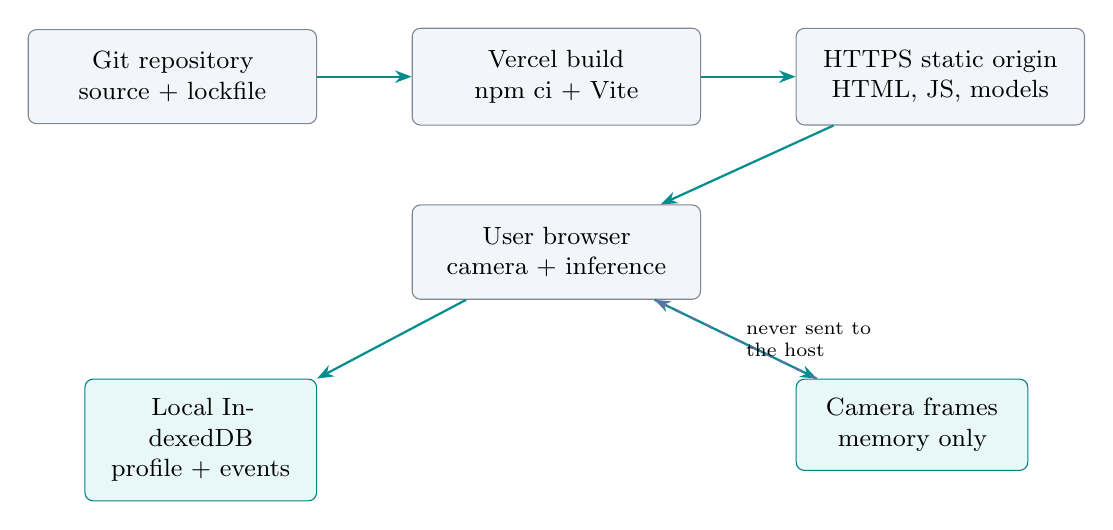
\begin{tikzpicture}[node distance=10mm and 12mm]
  \node[vboxwide] (git) {Git repository\\source + lockfile};
  \node[vboxwide,right=of git] (build) {Vercel build\\npm ci + Vite};
  \node[vboxwide,right=of build] (static) {HTTPS static origin\\HTML, JS, models};
  \node[vboxwide,below=of build] (browser) {User browser\\camera + inference};
  \node[vteal,below left=of browser] (data) {Local IndexedDB\\profile + events};
  \node[vteal,below right=of browser] (camera) {Camera frames\\memory only};
  \draw[vflow] (git) -- (build);
  \draw[vflow] (build) -- (static);
  \draw[vflow] (static) -- (browser);
  \draw[vflow] (browser) -- (data);
  \draw[vflow] (browser) -- (camera);
  \draw[vsoftflow] (camera) -- node[right,font=\scriptsize,align=left]{never sent to\\the host} (browser);
\end{tikzpicture}
\caption{Static Vercel deployment and local data boundary.}
\label{fig:deployment}
\end{figure}

The repository-root Vercel configuration rewrites client paths to `/index.html`, so a direct refresh on a page such as `/settings` can load the React router. Model assets use same-origin static paths and explicit caching headers. Camera APIs require a secure context; localhost and HTTPS are supported contexts in current browsers \cite{getUserMedia}. Deployment steps are: import the repository, select the root project, use `npm ci` and `npm run build`, set output to `dist`, define no environment variables, deploy, then verify an HTTPS camera prompt and direct-route refresh.

\chapter{Troubleshooting and Limitations}
\begin{longtable}{>{\raggedright\arraybackslash}p{0.24\textwidth}p{0.32\textwidth}p{0.36\textwidth}}
\caption{Practical troubleshooting reference.}\label{tab:troubleshooting}\\
\toprule
\textbf{Symptom} & \textbf{Likely cause} & \textbf{Action} \\
\midrule
\endfirsthead
\toprule
\textbf{Symptom} & \textbf{Likely cause} & \textbf{Action} \\
\midrule
\endhead
Camera stays off & Permission denied or non-secure origin & Use localhost or HTTPS; allow camera for the site, then press Start Vision. \\
No camera is listed & OS privacy restriction, disconnected device, or another app owns it & Check operating system camera privacy, close other camera clients, reconnect, reload, and reselect. \\
Models do not load & First-download network issue, blocked WASM/model asset, or storage cache issue & Verify same-origin asset requests, retry, update browser, and clear the model cache in Settings. \\
Face remains Unknown & No enrolled templates, low score, poor light/pose, or incompatible model template & Confirm consented enrollment on this browser, improve light/frontal angle, recapture quality-approved samples. \\
A result seems uncertain & Similar top identity scores or detector score near threshold & Preserve Unknown/ambiguous decision; do not use the output as an access decision. \\
Low frame rate & CPU/GPU load, large input, or slow backend & Choose Performance preset, reduce camera resolution, close heavy tabs, and inspect measured metrics. \\
QR does not validate & Invalid JSON/schema, duplicate ID, unsupported fields, or more than 8 KiB & Paste the decoded JSON into the form, check version 1/required fields, remove unsupported keys. \\
Saved data is absent & Different browser profile, private browsing, or storage was cleared & Return to the same browser/origin and profile. There is no account or cross-device sync. \\
Vercel deep link fails & Rewrite absent from deployed version & Redeploy `vercel.json` and confirm `/index.html` rewrite is active. \\
\bottomrule
\end{longtable}

When adjusting a recognition threshold, change it in small steps and use additional consented samples under realistic conditions. Raising a threshold generally makes matching stricter and increases Unknown outcomes. Lowering a threshold can make false matches more likely. Without a representative labeled evaluation set, neither value should be described as calibrated.

\section{Limitations}
The detector only recognizes the classes in its training vocabulary. The face model and matcher are sensitive to distance, illumination, occlusion, pose, motion blur, camera response, and shifts between training and use conditions. Browser runtimes differ in GPU and WASM support. Device memory and thermal constraints affect latency. Quality gates are heuristics rather than a spoof/liveness check. The current database is local to a browser origin/profile and is not synchronized or backed up automatically.

The recognition threshold and ambiguity margin are configurable initial values. The app has no population-scale verification protocol, no false-accept/false-reject study, and no fairness validation. A face descriptor can remain identifying personal data even though it is not a photograph. Browser storage can be removed by the user or browser cleanup. Profile exports intentionally omit biometric vectors, and camera frames are not included in any export.

There is also a model provenance boundary: the source of HSE FaceRes weights records training with VGGFace2, whose terms restrict the dataset to non-commercial research. The included asset is documented for local research/demo evaluation. Redistribution or commercial use requires a rights review or a replacement embedding model with compatible training-data rights. The code repository's MIT license does not establish third-party model rights.

\begin{cautionbox}
Do not use this demonstration for authentication, attendance enforcement, law enforcement, employment decisions, medical decisions, access control, or any other high-impact decision. A visual match is neither proof of liveness nor proof of a person's legal identity.
\end{cautionbox}

\chapter{Future Improvements}
Future work must be separated from what version 1 already does. The following items are not current features:
\begin{enumerate}
  \item \textbf{Replace or independently clear the face-model rights.} Select embedding weights with documented model and training-data terms for the intended deployment and evaluate them under a published consented protocol.
  \item \textbf{Calibrate the matcher.} Build a consented, demographically appropriate local evaluation set, define enrollment/query splits, and report false-match and false-nonmatch tradeoffs for the supported setting.
  \item \textbf{Encrypt user-controlled backups.} If cross-device portability is requested, design explicit key management and a user-consented encrypted export before introducing a sync service.
  \item \textbf{Offer more on-device model variants.} Compare size, license, latency, and detection quality with benchmark scripts and keep replacement models behind the same engine contract.
  \item \textbf{Improve accessibility validation.} Add screen-reader studies and keyboard-only camera workflows while preserving the explicit permission and stop states.
  \item \textbf{Extend tracking or cameras cautiously.} Multi-camera views and longer-lived tracking IDs would require a fresh threat model and a clear explanation of when identifiers persist.
\end{enumerate}

The architecture allows an alternate model adapter, a richer local evaluation harness, or another storage repository to be introduced without presenting those capabilities as if they already exist. Any future cloud synchronization or account feature would change the current privacy and deployment boundary and therefore needs a separate design decision.

\appendix
\chapter{Configuration Reference}
\begin{table}[htbp]
\centering
\caption{Selected starting configuration values. These values are not calibrated accuracy claims.}
\begin{tabularx}{\textwidth}{>{\raggedright\arraybackslash}p{0.33\textwidth}>{\raggedright\arraybackslash}p{0.19\textwidth}X}
\toprule
\textbf{Setting} & \textbf{Starting value} & \textbf{Effect} \\
\midrule
Object detector threshold & 0.50 & Filters COCO object scores below the selected value. \\
Face recognition threshold & 0.62 & Minimum normalized model-specific similarity for recognition. \\
Unknown match margin & 0.05 & Keeps close top identity candidates ambiguous. \\
Minimum approved samples & 3 & Enrollment requires several quality-approved face descriptors. \\
Maximum samples & 5 & Limits stored capture samples for one enrollment flow. \\
Balanced input & 640 by 480 & Maximum inference dimensions before resize. \\
Balanced cadence & 180 ms & Minimum interval between completed inference cycles. \\
Track expiry & 1800 ms & Removes tracks absent for the configured interval. \\
QR payload limit & 8192 bytes & Maximum UTF-8 payload size accepted by the parser. \\
\bottomrule
\end{tabularx}
\end{table}

\chapter{Reproducibility and Project Commands}
The source project is reproducible from its npm lockfile. On Windows, `setup.ps1` checks Node.js, runs `npm ci`, and performs a production build. To start a local development server, use `npm run dev`, then open the printed localhost URL. The core verification commands are:
\begin{lstlisting}
npm ci
npm run typecheck
npm run lint
npm test
npx playwright install chromium
npm run test:e2e
npm run build
npm run preview
\end{lstlisting}

To compile this PDF on a computer with MiKTeX or TeX Live containing XeLaTeX, Biber, TikZ, and the listed LaTeX packages, run \code{powershell -ExecutionPolicy Bypass -File docs/report/build-report.ps1}. The script performs the XeLaTeX/Biber passes and writes \code{output/pdf/VisionID\_AI\_Technical\_Report.pdf}. Render the pages with Poppler \code{pdftoppm} to inspect diagrams, tables, typography, and page flow.

\chapter{References}
The implementation report cites primary library, browser, hosting, and data terms documentation. Package versions and checked model assets are recorded in the repository lockfile and \code{docs/MODEL\_NOTICES.md}. Documentation links were verified on 3 October 2026.
\printbibliography[heading=none]

\end{document}
